\newpage

\section{Introduction}

% 此处介绍长周期彗星的背景,包括起源、活动性机制等,并在最后介绍两颗彗星样本相关信息

\begin{comment}
作为太阳系的原始天体,彗星具有着与早期太阳系行星系统相同的物理和化学性质,能够揭示有关早期太阳系的信息。研究彗星有利于我们进一步提高对行星形成机制认识,甚至可以解决诸如地球上水的起源等基本问题。

不同于短周期彗星,大部分长周期彗星起源于奥尔特云,而且是第一次进入太阳系。长周期彗星往往表现出比短周期彗星更强的活动性特征,在视觉上也会显得更为明亮,尤其是在近日点附近,会展现出极为壮观的爆发现象。这是因为长周期彗星含有更易挥发的组分,这些组分的升华效应会比常规的水冰升华效应更加显著。

长周期彗星在较大日心距的位置也会展现出较高的活动性,此时的活动性并非由水冰升华效应导致的,目前的解释主要有以下几个部分:非晶态和晶态水冰之间的相变\citep{prialnik_crystallization_1992, capria_c1995_2002},非晶态水冰的退火\citep{meech_activity_2009},以及CO和/或CO2等更易挥发组分的升华。对于在日心距超过4AU 处活动且彗核表面温度低于H2O升华温度的彗星,其活动可能由更易挥发的CO2(已由AKARI 观测确定,\citealp{ootsubo_akari_2012})或CO\citep{jewitt_distant_2019}的升华造成的。此外,\citet{ivanova_observations_2011}的相关研究还表明,为符合彗星长期高活动性的观测结果,彗核的上层会不断剥离。

% 有关图像增强的部分放到后面

在大部分情况下,彗星的彗发结构是较难直接观测得到的,往往只是比背景有细微的差别,需要通过一系列的图像增加技术加以区分。关于这方面的研究较为丰富,比如,Manzini 等(2007)、Szabó 等(2001, 2008)、Meech 等(2009)、Mazzotta Epifani 等(2009)、Shubina 等(2014)、Korsun 等(2006, 2016)、Ivanova 等(2011)和Kulyk 等(2016, 2018, 2021)曾对几种彗星的观测结果应用图像增强方法进行分析,并据此计算相关物理参数。

本文对两颗长周期彗星C/2019 L3与C/2020 P3的活动性与相关物理性质进行了研究,它们的轨道根数如表~\ref{tab:orb_elem}~所示,这两颗彗星的半长轴a大于10000AU,Nearly isotropic。根据获取的观测图像文件,通过孔径测光的方法计算出两者的BVR三个波段的星等,基于测光结果计算了对应的色指数、经过相位角校正的$Af\rho$以及表面亮度轮廓信息。
\end{comment}

As primitive objects in the Solar System, comets have the same physical and chemical properties as the planetary systems in the early Solar System, which can reveal information about the early Solar System. Research on comets can let us further understand the mechanism of planet formation and even solve some basic questions such as the origin of water on Earth. Unlike \st{short-period} \ul{Short-peroid} comets \ul{($\rm P<\SI{200}{yr}$)}, most \st{long-period} \ul{Long-period} comets \ul{($\rm P>\SI{200}{yr}$)} originate from the Oort Cloud and are entering the \ul{inner} Solar System for the first time. Long-period comets tend to exhibit stronger activity characteristics than \st{short-period} \ul{Short-peroid} comets do and appear brighter visually due to the more volatile components they contain, comparing with the conventional water ice. 

Long-period comets also exhibit \st{high} activity at large heliocentric distances \ul{more than {\SI{5}{\astronomicalunit}}}. At this time, the activity is not caused by the sublimation effect of water ice. The current explanation \ul{about distant activity of comets} mainly includes \st{the following parts}: the phase transition between amorphous and crystalline water ice \citep{prialnik_crystallization_1992, capria_c1995_2002}, the annealing of amorphous water ice \citep{meech_activity_2009}, and the sublimation of more volatile components such as \ce{CO2}~\citep{ootsubo_akari_2012} and/or \ce{CO}~\citep{jewitt_distant_2019}. 
% For comets that are active at a heliocentric distance of more than {\SI{4}{\astronomicalunit}} and whose nucleus surface temperature is lower than the \ce{H2O} sublimation temperature, their activity may be caused by the sublimation of more volatile \ce{CO2}~\citep{ootsubo_akari_2012} or \ce{CO}~\citep{jewitt_distant_2019}. In addition, \citet{ivanova_observations_2011} show that the upper layer of the comet nucleus should continue to peel off in order to conform to the observation results of long-term high activity of comets. 

Two \st{long period} \ul{Long-period} comets C/2019 L3 and C/2020 P3 are selected for this study. They are all nearly isotropic, both of them having orbital semi-major axis more than {\SI{10000}{\astronomicalunit}}. C/2019 L3 and C/2020 P3 reach their perihelion on \DTMdate{2022-1-9} and \DTMdate{2021-4-21}. \autoref{fig:orbit} shows the planar orbit graph of them in Solar System. \autoref{tab:orb_elem} is the summary on orbital elements of these two comets. 

In this paper, we present \st{several observational} \ul{broadband CCD photometry} results of the two comets metioned above. \st{We present the} \ul{The} circumstance of observations and data reduction process \ul{are presented} in section \ref{sec:obs_data}. Section \ref{sec:res} describes the \st{data analysis} \ul{photometry} results, including morphology, \st{photometry,} surface brightness, $Af\rho$ and coma colors. Finally, discussion and conclusions are presented in section \ref{sec:dis} and section \ref {sec:con}. 

% orbital graph
\begin{figure}
    \centering
    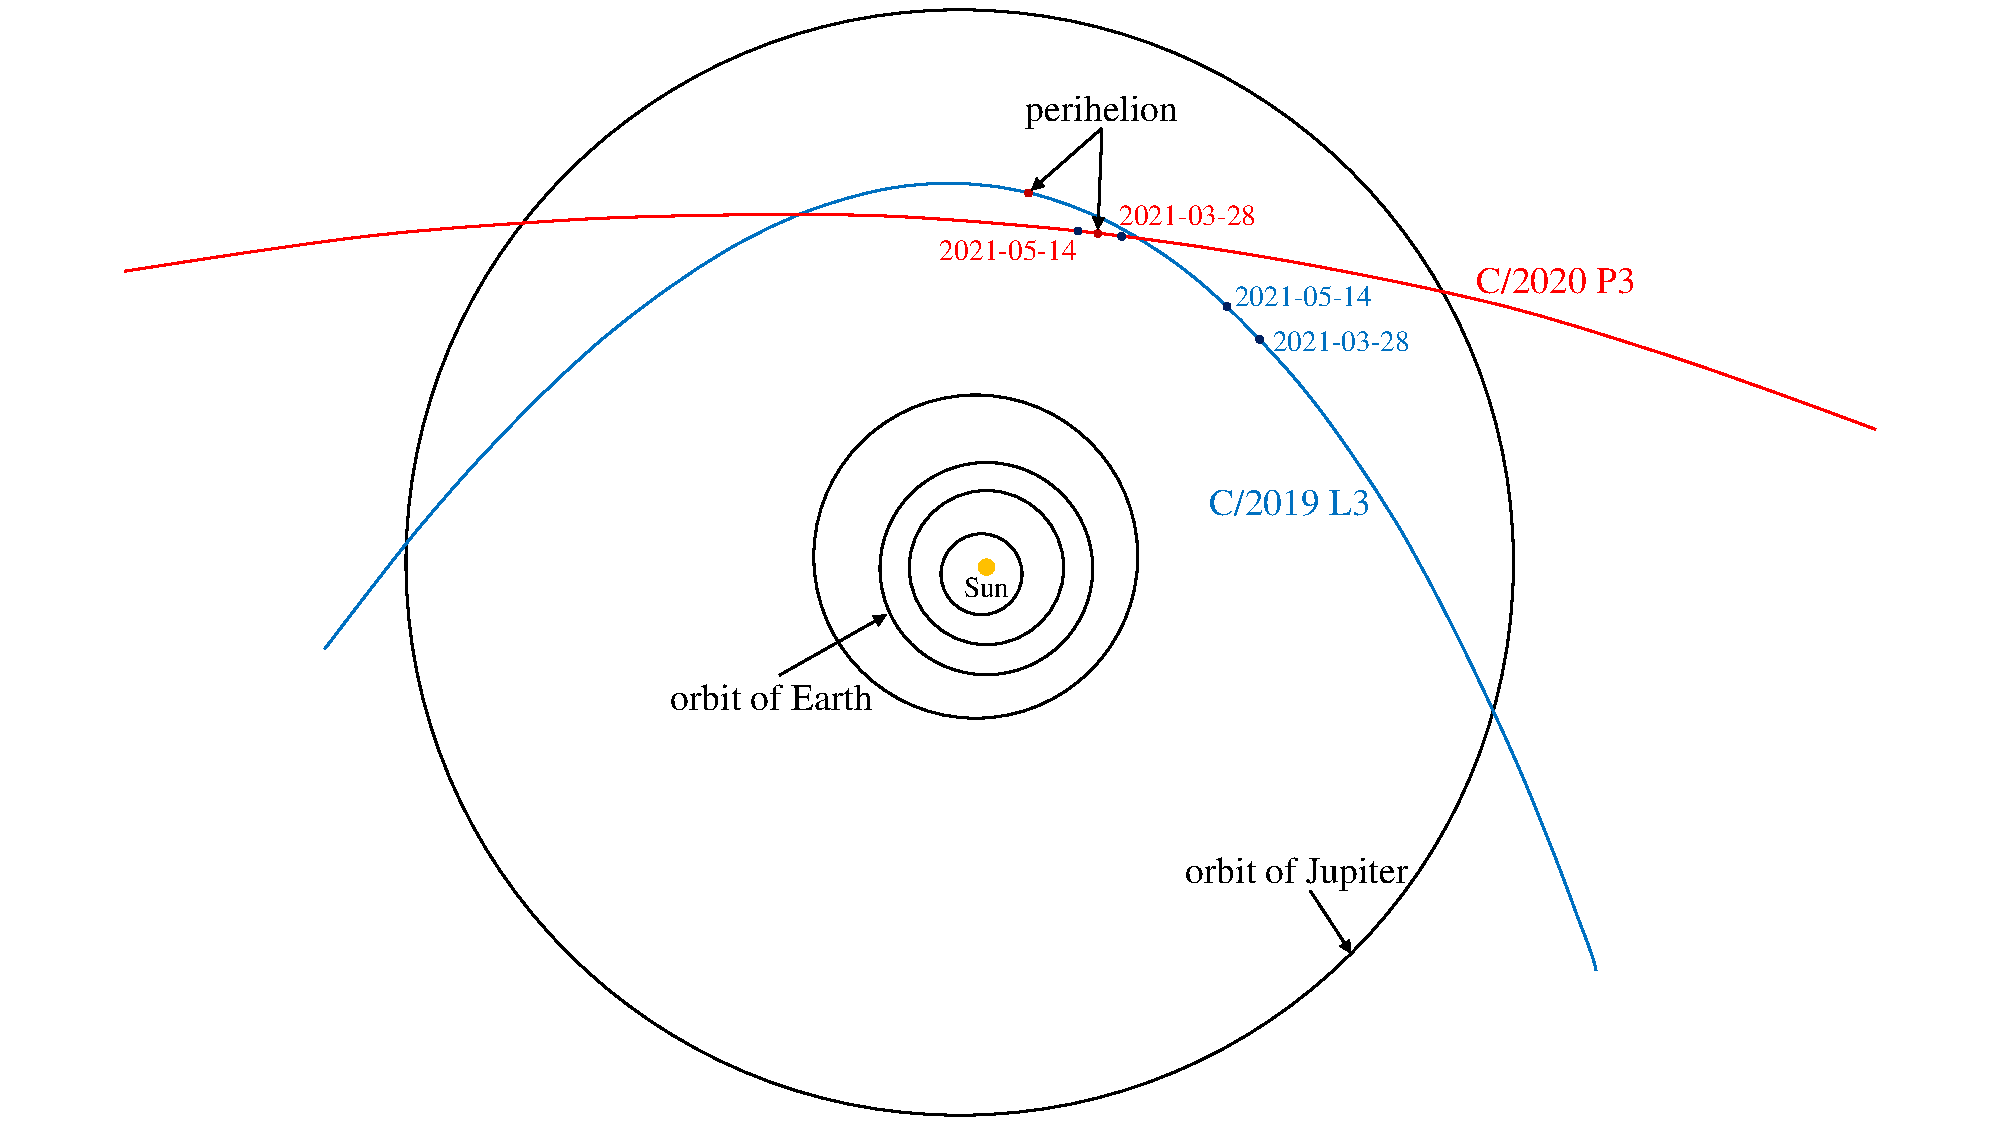
\includegraphics[width=1.0\columnwidth]{orbit.pdf}
    \caption{Orbit of \st{two} comets \ul{C/2019 L3 and C/2020 P3} in \ul{the} Solar System. The blue curve is the orbit of C/2019 L3 and the red curve is the orbit of C/2020 P3. Closed curves in black are the orbits of planets in \ul{the} Solar System. Note that both of these comets have large orbital inclination not shown in this planar graph. The start and end dates of observations as well as the corresponding position of two objects on these dates are marked in this graph. }
    \label{fig:orbit}
\end{figure}

% orbital elements
\begin{table}[!htbp]
    \centering
    \caption{Orbital elements of \st{two} comets \ul{C/2019 L3 and C/2020 P3} (Epoch: Jul 19 2022). }\label{tab:orb_elem}
    \begin{threeparttable}
        \resizebox{\linewidth}{!}{
        \begin{tabular}{ccccccccc}
            \toprule
            Comet \tnote{0} & e\tnote{1} & q\tnote{2} & i\tnote{3} & $\Omega$\tnote{4} & $\omega$\tnote{5} & L\tnote{6} & B\tnote{7} & T\tnote{8} \\
            \midrule
            C/2019 L3       & \num{1.0017730}  & \num{3.5544290}  & \num{48.35710}  & \num{290.78850}  & \num{171.60970}  & \num{285.19094}  & \num{6.26014}   & \num{2459589.11650}  \\
            C/2020 P3       & \num{1.0003270}  & \num{6.8123330}  & \num{61.88790}  & \num{19.46850}   & \num{82.25590}   & \num{93.37021}   & \num{60.92485}  & \num{2459325.45200} \\
            \bottomrule
        \end{tabular}
        }
% 在正文介绍classification的部分
        \begin{tablenotes}
            \item[0] \st{data resource: }\href{http://astro.vanbuitenen.nl/}{\st{astro.vanbuitenen.nl}}
            \item[1] eccentricity 
            \item[2] perihelion distance
            \item[3] inclination
            \item[4] Longitude of ascending node
            \item[5] Argument of perihelion
            \item[6] Longitude of perihelion
            \item[7] Latitude of perihelion
            \item[8] Time of perihelion passage
        \end{tablenotes}
    \end{threeparttable}
\end{table}
